% Seccion «Algoritmo implementado» (entrega final). Se incluye desde sn-article.tex.
% Los numeros se reproducen desde backend/ con los comandos de docs/GUIA.md.

El algoritmo se implementó en Python como el paquete \texttt{asignador}, independiente de la web, siguiendo los TADs de la Sección~\ref{sec:tads} y la formalización de la Sección~\ref{sec:formal}. Los diez niveles de la Tabla~\ref{tab:niveles} están implementados y son acumulativos: cada nivel se puede ejecutar por separado para comparar resultados. Esta sección explica su desarrollo y funcionamiento (Sección~\ref{sec:impl}), las estrategias algorítmicas utilizadas y dónde se aplican (Sección~\ref{sec:estrategias}) y el análisis de su complejidad temporal (Sección~\ref{sec:complejidad}); al final se resumen las pruebas y resultados que lo respaldan (Sección~\ref{sec:resultados}).

\subsection{Desarrollo y funcionamiento}\label{sec:impl}

\subsubsection{Estructura del código}

\begin{table}[htbp]
\caption{Módulos principales del paquete \texttt{asignador}}\label{tab:modulos}
\small
\begin{tabularx}{\textwidth}{@{}lL@{}}
\toprule
Módulo & Responsabilidad \\
\midrule
\texttt{dominio/} & TADs de entrada inmutables: Franja, Sesión, Sección, Materia, Estudiante, Solicitud, Preferencias \\
\texttt{datos/} & Lectura de los JSON y validación de precondiciones; informa archivo, registro, campo y error \\
\texttt{algoritmo/horario.py} & TAD Horario: \emph{puedeAgregar}, \emph{agregar}, \emph{quitar}; los inscritos por sección son estado de la corrida \\
\texttt{algoritmo/reglas.py} & R2--R8 como objetos intercambiables; cada nivel activa las suyas (R1 y R9 se cumplen por construcción) \\
\texttt{algoritmo/voraz.py} & Orden de atención y asignación voraz (N1--N9); avisos con causa y sugerencia \\
\texttt{algoritmo/eleccion.py} & Elección entre secciones válidas (N5--N9) \\
\texttt{algoritmo/mejora.py} & Desempate por semestre y mejora local (N10) \\
\texttt{satisfaccion.py} & Los cinco criterios de la Sección~\ref{sec:metricas} y su promedio ponderado \\
\texttt{objetivo.py} & El orden completo de la Sección~\ref{sec:objetivo} para comparar resultados \\
\texttt{verificador.py} & Recalcula R1--R9 sobre la salida guardada, sin reutilizar código del algoritmo \\
\texttt{exacto.py} & Solución exacta por búsqueda exhaustiva para instancias pequeñas \\
\texttt{generador/} & Instancias sintéticas reproducibles por semilla, grandes y pequeñas \\
\botrule
\end{tabularx}
\end{table}

Una corrida lee y valida los datos, ejecuta el nivel pedido, serializa la salida en el formato de la Sección~\ref{sec:datos}, la pasa por el verificador, calcula las métricas y guarda todo en \texttt{resultados/}, junto con una copia de las entradas usadas. El servidor FastAPI y la línea de comandos llaman a la misma función.

\subsubsection{Cómo funciona cada nivel}

\paragraph{N1--N4: voraz por prioridad.} Todas las solicitudes se ordenan de mayor a menor prioridad y, a igual prioridad, por código de estudiante y de materia, para que el resultado no dependa del orden de los registros en los JSON. Cada solicitud toma la primera sección, en orden de identificador, que cumple las reglas del nivel. Desde N4, si ninguna sección de la principal cabe, se prueban las sustitutas en el orden de su lista; la sustituta hereda la prioridad de la solicitud. El aviso registra todas las causas y destaca la más frecuente entre las secciones de la principal (Sección~\ref{sec:fallos}).

\paragraph{N5--N9: elección por satisfacción.} Entre las secciones válidas se elige la mejor según este orden:
\begin{enumerate}
\item la menor pérdida en las solicitudes que al mismo estudiante le quedan por atender, comparada de prioridad 5 a 1: una solicitud que se queda sin ninguna sección posible pierde 1, y una que solo podría entrar por sustituta pierde 0,2;
\item la mayor satisfacción con los criterios del nivel: profesores (N5), más horario y huecos (N6), más cercanía (N7); hasta N7 con los pesos por defecto y desde N8 con la importancia declarada; en N9 se agregan los compañeros y se suma también la satisfacción de quienes tienen afinidad hacia el estudiante;
\item el menor identificador de sección.
\end{enumerate}
Cada candidata se mide inscribiéndola de forma provisional con \emph{agregar} y retirándola con \emph{quitar}.

\paragraph{N10: desempate por semestre y mejora local.} El voraz de N9 se ejecuta primero; si el desempate por semestre está activo, a igual prioridad se atiende antes al estudiante de mayor semestre. Después se hacen pasadas de mejora con dos tipos de cambio: (1) para cada solicitud no atendida por su principal, inscribir la principal (o, si está pendiente, una sustituta), moviendo si hace falta a un ocupante de la sección llena a otra sección de la misma materia con cupo; y (2) pasar cualquier inscripción a otra sección de la misma materia. Un cambio se acepta solo si mejora estrictamente el resultado según la Sección~\ref{sec:objetivo}; se examinan como máximo \texttt{max\_cambios} cambios. Al final los avisos se recalculan con el horario definitivo.

\subsubsection{Fragmentos del código}\label{sec:codigo}

Los listados siguientes son extractos del paquete \texttt{asignador} (ligeramente acortados). Muestran las tres piezas que definen el recorrido: ordenar y asignar solicitudes, elegir entre secciones válidas, y mejorar con desplazamientos. No se ejecutan los diez niveles en cadena: cada corrida usa un solo nivel; N10 parte de cero con el voraz completo y luego aplica la mejora.

\paragraph{Orden y bucle voraz.} Una solicitud es el pedido de un estudiante por una materia (código, prioridad 1--5 y, opcionalmente, sustitutas). El algoritmo no llena salones de arriba a abajo: aplana todas las solicitudes, las ordena y, para cada una, intenta inscribir a \emph{ese} estudiante en alguna sección de \emph{esa} materia. Hasta N4 toma la primera válida; desde N5 delega en el elector. Si la principal no cabe y el nivel admite sustitutas, las prueba en orden (Listado~\ref{lst:voraz}).

\begin{lstlisting}[style=python,caption={Orden de atenci\'on y bucle voraz (\texttt{voraz.py})},label={lst:voraz}]
def orden_de_atencion(instancia, por_semestre=False):
    pares = [(e, s) for e in instancia.estudiantes.values()
             for s in e.solicitudes]
    return sorted(pares, key=lambda par: (
        -par[1].prioridad,
        -par[0].semestre if por_semestre else 0,  # solo N10
        par[0].id, par[1].materia))

def asignar_voraz(instancia, nivel):
    orden = orden_de_atencion(instancia, usa_semestre(instancia, nivel))
    # ... crea horarios y cola de pendientes por estudiante ...
    for estudiante, solicitud in orden:
        candidatas = instancia.secciones_de(solicitud.materia)
        if inscribir(candidatas):          # principal
            continue
        if nivel.sustitutas:               # desde N4
            for codigo in solicitud.sustitutas:
                if inscribir(instancia.secciones_de(codigo)):
                    break
        # si nada cupo: aviso con causas
\end{lstlisting}

\paragraph{Elección entre secciones válidas (N5--N9).} Cuando hay varias secciones que cumplen las reglas, no se elige solo por comodidad. Cada candidata se inscribe de forma provisional (\emph{agregar}/\emph{quitar}): primero se mide cuánto daña las solicitudes que al mismo estudiante aún le faltan (prioridad 5 a 1); solo después entra la satisfacción del nivel; al empatar, el menor identificador (Listado~\ref{lst:eleccion}).

\begin{lstlisting}[style=python,caption={Puntaje al elegir secci\'on (\texttt{eleccion.py})},label={lst:eleccion}]
def mejor(self, horario, solicitud, validas, pendientes):
    return max(validas, key=lambda s: self._puntaje(
        horario, Inscripcion(solicitud, s), pendientes))

def _puntaje(self, horario, inscripcion, pendientes):
    horario.agregar(inscripcion)           # prueba
    try:
        perdidas = self._perdidas(horario, pendientes)  # prio 5..1
        total = self.satisfaccion(horario.estudiante.id)
        # en N9 tambien suma la de quienes tienen afinidad hacia el
    finally:
        horario.quitar(inscripcion)        # deshace
    # max() gana con el mayor: se niegan las perdidas
    return tuple(-p for p in perdidas), total
\end{lstlisting}

\paragraph{Mejora local (N10).} Tras el voraz, se recorren primero las solicitudes no atendidas por su principal y luego reubicaciones a otra sección de la misma materia. Si el único obstáculo es el cupo, se intenta mover a un ocupante a otra sección con cupo y meter al que faltaba. Cada intento se acepta solo si la parte tocada de $Q$ mejora estrictamente; si no, se deshace (Listado~\ref{lst:mejora}).

\begin{lstlisting}[style=python,caption={Pasadas de mejora y desplazamiento (\texttt{mejora.py})},label={lst:mejora}]
def ejecutar(self):
    while mejoro and not self.agotado:     # tope: max_cambios
        mejoro = False
        for estudiante, solicitud in orden:
            mejoro |= self._mejorar_solicitud(...)  # insertar
        for eid, insc in inscripciones:
            mejoro |= self._mejorar_seccion(...)    # reubicar

def _intentar(self, eid, solicitud, actual, seccion):
    causas = self._causas_sin(horario, actual, seccion)
    if not causas:
        return self._probar([quitar_actual, agregar_nueva])
    if causas != [Causa.CUPO_LLENO]:
        return False
    # desplazar a un ocupante a otra seccion de la misma materia
    for otro in sorted(ocupantes[seccion.id]):
        for alternativa in alternativas_con_cupo:
            if self._probar([mover_otro, quitar_actual, agregar_nueva]):
                return True
    return False
\end{lstlisting}

\subsubsection{Decisiones tomadas al implementar}\label{sec:decisiones}

\begin{itemize}
\item \textbf{Revisar las solicitudes pendientes antes que la satisfacción (N5--N9).} Elegir solo por satisfacción podía hacer que una sección cómoda chocara con otra materia del mismo estudiante, en contra de la Sección~\ref{sec:objetivo} (caso ``Preferencias'' de la Tabla~\ref{tab:aceptacion}). Esta revisión además subió la cobertura de 85,6~\% (N4) a 88,2~\% (N5) en la instancia de la Sección~\ref{sec:resultados}.
\item \textbf{Suma de posiciones de sustitutas desde 1.} La primera sustituta de una lista cuenta 1 y no 0; así, entre dos resultados que empatan en $C_k$, gana el que usa menos sustitutas.
\item \textbf{Dos causas nuevas en la Tabla~\ref{tab:causas}.} ``Materia ya inscrita'', cuando una sustituta común a dos solicitudes ya atendió la otra, y ``Limitación del algoritmo'', cuando una sección cabía en el horario final y no se tomó, como pide la Sección~\ref{sec:fallos}.
\item \textbf{``Cedida por prioridad''} se informa solo en N10 con el desempate activo, cuando el cupo lo tiene alguien con la misma prioridad y mayor semestre.
\item \textbf{Comparaciones sin errores de redondeo.} Las sumas de $Q$ se redondean a nueve decimales (cinco sustituciones de 0,8 deben empatar con cuatro principales) y la satisfacción se suma sin el redondeo a cuatro decimales de la salida.
\item \textbf{La mejora de N10 solo acepta mejoras reales}: debe mejorar $C$, $J$, la satisfacción o las sustitutas; el último desempate por códigos no basta para aceptar un cambio.
\item \textbf{Solución exacta propia en lugar de CP-SAT.} La Sección~\ref{sec:datos} admitía revisar todas las combinaciones válidas; se eligió esa opción para no depender de bibliotecas nativas. La búsqueda comprueba las reglas con su propio código.
\item \textbf{El verificador revisa R1--R9 en todos los niveles.} Los niveles que aún no aplican una regla muestran sus violaciones como ``no aplica'', lo que permite ver qué agrega cada nivel.
\item \textbf{Cambios respecto a la Tabla~\ref{tab:tec}.} La solución exacta se hizo con una búsqueda propia en lugar de OR-Tools CP-SAT (punto anterior). El sistema se ejecuta localmente con \texttt{dev.sh} o \texttt{dev.ps1}; Docker Compose y la integración continua quedaron como trabajo futuro. Se agregó \texttt{traslados.json} a los datos de entrada, con los minutos de caminata entre edificios.
\end{itemize}

\subsubsection{Aplicación implementada}

La aplicación web (React con TypeScript) sigue el recorrido y el aspecto de los diseños de la Sección~\ref{sec:ui} y llama al mismo paquete a través del servidor FastAPI. Permite cargar o generar datos (con respaldo previo en \texttt{data/.respaldos/}), editar las preferencias de cada estudiante con validación en el servidor (si hay errores no escribe nada y los muestra junto a su campo), ejecutar cualquier nivel o las referencias, activar el desempate por semestre solo para una corrida, comparar todos los niveles sobre los mismos datos y consultar el horario de cada estudiante con sus sustituciones, avisos y satisfacción por criterio (Figuras~\ref{fig:app-resultados} y~\ref{fig:app-horario}).

\begin{figure}[htbp]
\centering
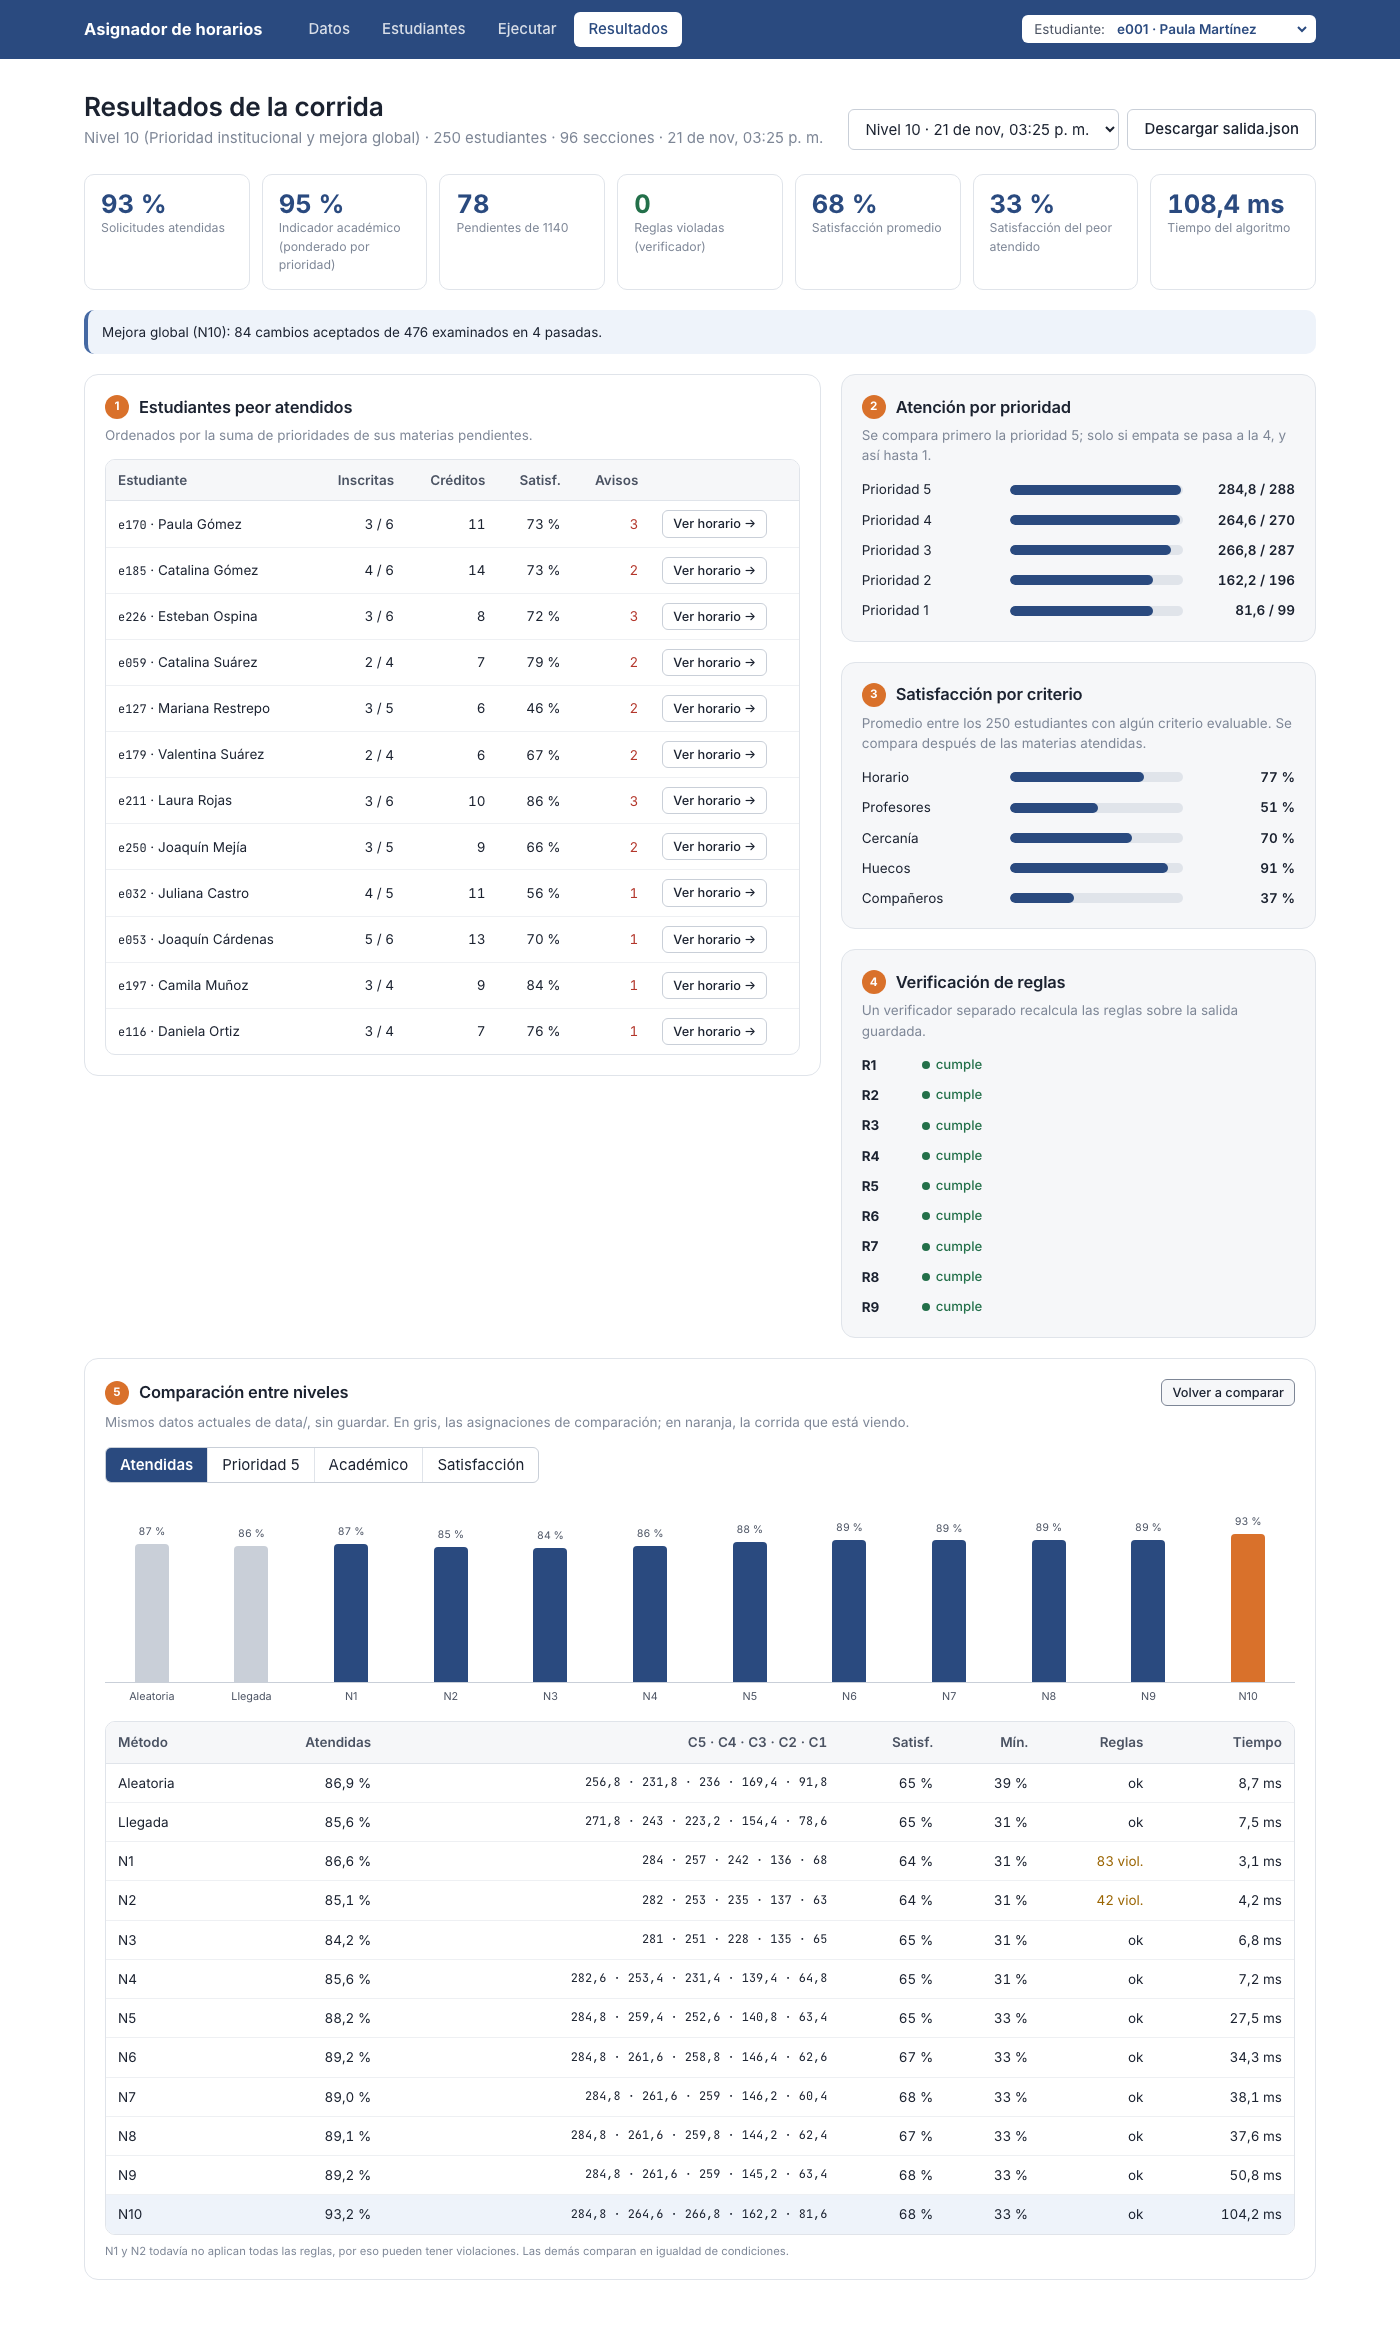
\includegraphics[width=0.7\textwidth]{figuras/app_resultados.png}
\caption{Aplicación: resultados de N10, satisfacción por criterio, verificación de reglas y comparación entre niveles.}\label{fig:app-resultados}
\end{figure}

\begin{figure}[htbp]
\centering
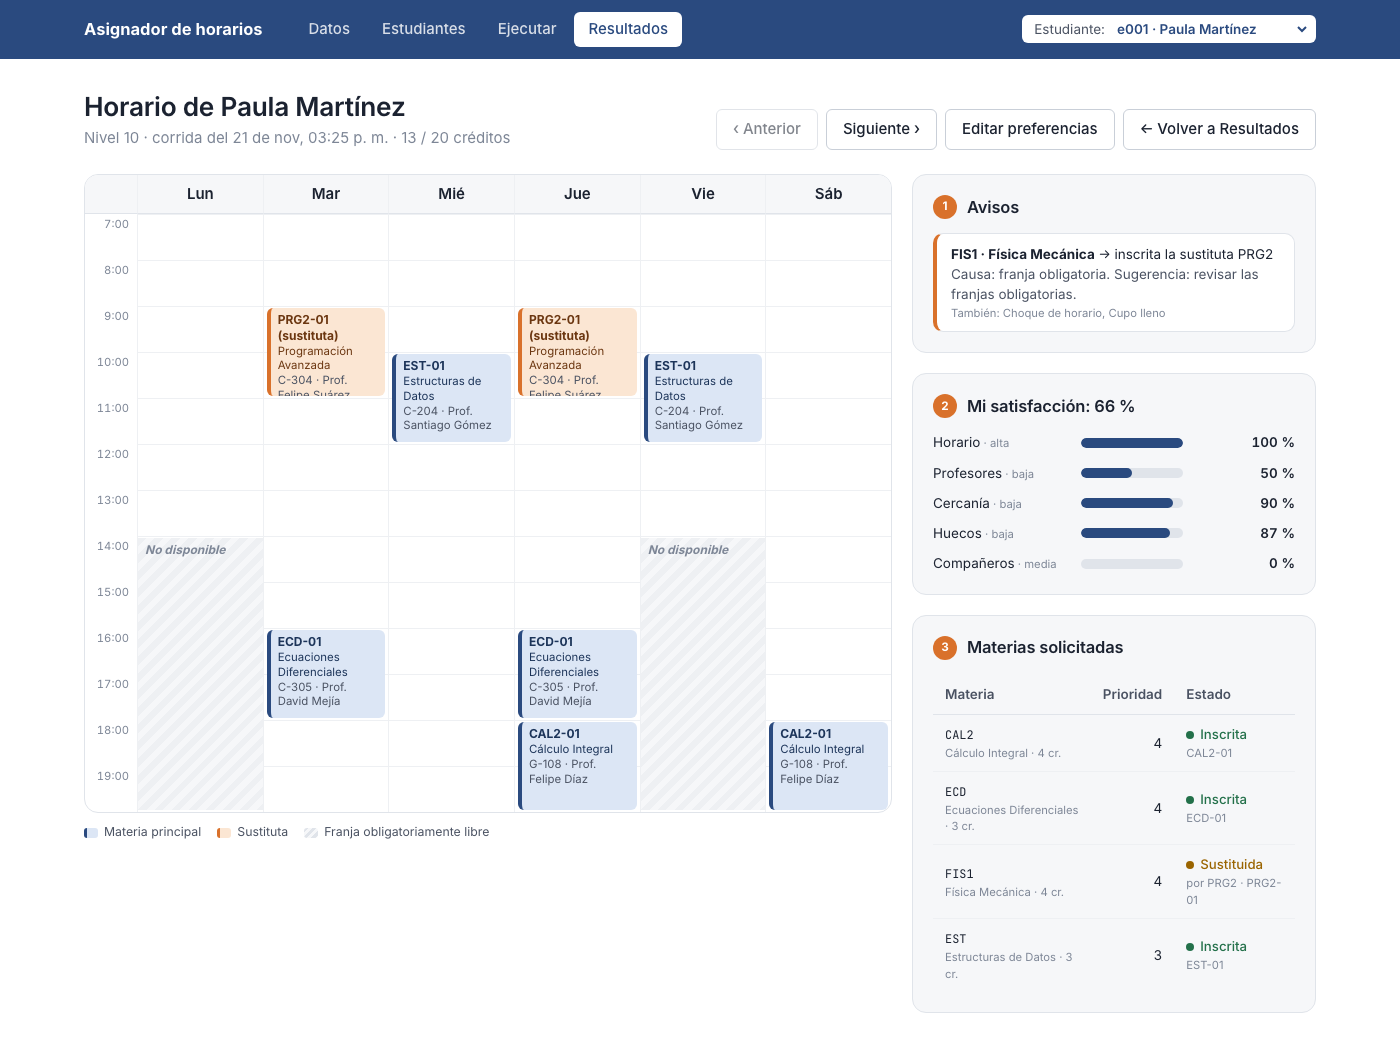
\includegraphics[width=\textwidth]{figuras/app_horario.png}
\caption{Aplicación: horario de un estudiante con una sustitución, su aviso y su satisfacción por criterio.}\label{fig:app-horario}
\end{figure}

\subsection{Estrategias algorítmicas}\label{sec:estrategias}

La solución combina varias estrategias. La Tabla~\ref{tab:estrategias} indica dónde se aplica cada una y los párrafos siguientes explican cómo y por qué. Las cuatro primeras forman el algoritmo entregado (N10); las demás se usan para evaluarlo.

\begin{table}[htbp]
\caption{Estrategias algorítmicas y dónde se aplican}\label{tab:estrategias}
\small
\begin{tabularx}{\textwidth}{@{}>{\raggedright\arraybackslash}p{0.3\textwidth}Ll@{}}
\toprule
Estrategia & Dónde se aplica & Archivo \\
\midrule
Ordenamiento previo & Orden de atención de todas las solicitudes (N1--N10) & \texttt{voraz.py} \\
Voraz por prioridad & Asignación de N1--N9 y punto de partida de N10 & \texttt{voraz.py} \\
Voraz con mirada adelante & Elección entre secciones válidas (N5--N9) & \texttt{eleccion.py} \\
Búsqueda local con evaluación incremental & Mejora de N10 & \texttt{mejora.py} \\
Vuelta atrás con poda & Solución exacta para comparar (instancias pequeñas) & \texttt{exacto.py} \\
Aleatorización y construcción inversa & Referencia aleatoria, generador y casos con respuesta conocida & \texttt{referencias.py}, \texttt{generador/} \\
\botrule
\end{tabularx}
\end{table}

\paragraph{Ordenamiento previo.} Antes de asignar, las $R$ solicitudes de todos los estudiantes se ordenan con la clave (prioridad descendente; semestre descendente, solo en N10 con el desempate activo; código del estudiante; código de la materia). El ordenamiento cumple dos funciones: fija qué se atiende primero, de acuerdo con el orden de la Sección~\ref{sec:objetivo}, y hace el resultado determinista, porque no depende del orden de los registros en los JSON. Esta última propiedad se comprueba en las pruebas barajando los archivos de entrada.

\paragraph{Voraz por prioridad (N1--N9).} Se recorren las solicitudes ya ordenadas y cada una toma una sección en ese momento, sin volver atrás: hasta N4 la primera que cumple las reglas del nivel y, desde N5, la mejor de las válidas. Si ninguna sección de la principal cabe, se prueban las sustitutas en el orden de su lista. Se eligió esta estrategia porque el orden de la Sección~\ref{sec:objetivo} compara primero $C_5$: si todas las solicitudes de prioridad 5 eligen antes que las demás, ninguna solicitud de menor prioridad puede quitarles un cupo. Cada decisión es local y no se deshace, y por eso el voraz no garantiza el óptimo. Por ejemplo, si una sección $S_1$ tiene un solo cupo, el estudiante $a$ puede usar $S_1$ o $S_2$ y el estudiante $b$ solo $S_1$, entonces $a$, que se atiende primero, toma $S_1$ y $b$ queda sin la materia. N10 corrige este caso.

\paragraph{Voraz con mirada adelante (N5--N9).} Entre las secciones válidas de una solicitud no se toma solo la más cómoda. Primero se mira un paso adelante: para cada candidata se calcula cuántas de las solicitudes que al mismo estudiante le quedan por atender dejarían de caber (cada una pierde 1, o 0,2 si solo podría entrar por sustituta), comparando de prioridad 5 a 1. Solo entre las candidatas que empatan en esa pérdida se usa la satisfacción, y al final el menor identificador. Para medir cada candidata se usa la técnica de \emph{prueba y deshacer}: se inscribe de forma provisional con \emph{agregar} del TAD Horario, se mide y se retira con \emph{quitar}, sin copiar el estado. Esta regla evita que una sección cómoda bloquee otra materia del mismo estudiante y subió la cobertura de 85,6~\% (N4) a 88,2~\% (N5).

\paragraph{Búsqueda local (N10).} Parte de la solución del voraz y explora soluciones vecinas con dos movimientos:
\begin{enumerate}
\item \emph{Insertar con desplazamiento}: una solicitud no atendida por su principal intenta entrar en una sección de su principal (o, si está pendiente, en una sustituta). Si esa sección solo está bloqueada por el cupo, uno de sus ocupantes se mueve a otra sección de la misma materia que tenga cupo. Es la corrección del ejemplo anterior: $a$ pasa a $S_2$ y $b$ entra en $S_1$.
\item \emph{Reubicar}: una inscripción pasa a otra sección de la misma materia, si eso mejora la satisfacción sin perder materias.
\end{enumerate}
Se acepta el primer movimiento que mejora \emph{estrictamente} el orden de la Sección~\ref{sec:objetivo} (estrategia de ascenso por primera mejora); si no mejora, se deshace. Como cada cambio aceptado mejora estrictamente el puntaje y el número de asignaciones es finito, no se repite ninguna asignación y el proceso termina. Para acotar el tiempo se examinan como máximo $M$ cambios (\texttt{max\_cambios}). Para comparar no se recalcula el puntaje de todos los estudiantes: solo cambia el aporte de los dos estudiantes que se mueven y la satisfacción de ellos y de quienes tienen afinidad hacia ellos, y como el orden se compara componente a componente, basta con comparar esa parte (\emph{evaluación incremental}). Así, cada cambio cuesta $O(r^2 + (1+I)\,c_S)$ en lugar de $O(E\,c_S)$. La búsqueda local encuentra un óptimo local respecto a esos dos movimientos, no el global: las mejoras que requieren tres o más cambios coordinados no se exploran (Sección~\ref{sec:limitaciones}).

\paragraph{Vuelta atrás con poda (solución exacta).} Para saber qué tan lejos queda N10 del óptimo, \texttt{exacto.py} recorre con vuelta atrás (\emph{backtracking}) todas las asignaciones válidas: cada solicitud puede quedar en una sección de su principal, en una de sus sustitutas o pendiente, y se descartan de inmediato las ramas que violan alguna regla. Se poda una rama cuando su vector optimista (lo ya atendido más todas las solicitudes restantes contadas como principales) es estrictamente peor que el de la mejor solución encontrada (ramificación y acotamiento). La poda nunca descarta una rama que pueda empatar en $C$, porque podría ganar por $J$ o por satisfacción; así el resultado sigue siendo óptimo. Su costo es exponencial (Sección~\ref{sec:complejidad}), por lo que solo se usa en instancias de 2 a 6 estudiantes. Comprueba las reglas con su propio código, sin reutilizar el del algoritmo.

\paragraph{Aleatorización y construcción inversa (evaluación).} La referencia aleatoria baraja las solicitudes y las secciones con Fisher--Yates usando una semilla, de modo que sus resultados son reproducibles. El generador de instancias también depende solo de la semilla. Para los casos con respuesta conocida se invierte el problema: primero se construye una asignación válida para todos y después se derivan de ella las solicitudes y los cupos. Así se conoce un resultado que atiende el 100~\% sin tener que resolver el problema, lo que sirve para instancias medianas donde la búsqueda exhaustiva ya no es viable.

\paragraph{Reglas como filtros intercambiables.} Las reglas R2--R8 se implementaron como objetos con la misma interfaz, y cada nivel es una lista de reglas activas más unas banderas (sustitutas, criterios de satisfacción, mejora). \emph{puedeAgregar} aplica los filtros y devuelve la lista de causas por las que una sección no cabe; esa misma lista alimenta los avisos, que cuentan las causas y destacan la más frecuente. Esto permite agregar un nivel sin tocar el voraz y ejecutar cualquier nivel por separado para comparar.

\subsection{Análisis de complejidad}\label{sec:complejidad}

Esta sección analiza el tiempo y la memoria de la implementación entregada, nivel por nivel, y contrasta el análisis con mediciones. Los costos se expresan con los parámetros de la Tabla~\ref{tab:notacion}; los que dependen de un solo estudiante están acotados por los datos (por ejemplo, con 20 créditos y materias de al menos 1 crédito, nadie inscribe más de 20 materias), mientras que $E$, $R$ y $\sigma$ crecen con el tamaño de la universidad.

\begin{table}[htbp]
\caption{Notación del análisis}\label{tab:notacion}
\small
\begin{tabularx}{\textwidth}{@{}lL@{}}
\toprule
Símbolo & Significado \\
\midrule
$E$, $S$ & Número de estudiantes y de secciones \\
$R$ & Total de solicitudes ($R \le r\,E$) \\
$r$ & Máximo de solicitudes de un estudiante \\
$\sigma$ & Máximo de secciones de una materia \\
$\beta$ & Máximo de sustitutas de una solicitud \\
$q$ & Máximo de sesiones de una sección \\
$f$, $F$ & Franjas obligatorias y franjas de preferencia de un estudiante (con \texttt{*} expandido a seis días) \\
$\alpha$, $I$ & Preferencias sociales de un estudiante y estudiantes con afinidad hacia uno dado \\
$c$ & Máximo cupo de una sección \\
$M$ & Límite de cambios examinados en N10 (\texttt{max\_cambios}, 10.000 por defecto) \\
\botrule
\end{tabularx}
\end{table}

\subsubsection{Operaciones básicas}

\paragraph{Comprobar las reglas.} \emph{puedeAgregar} evalúa R2--R8 sobre el horario del estudiante. R2 y R5 recorren sus inscripciones, $O(r)$; R3 compara cada sesión nueva con cada sesión inscrita, $O(r q^2)$; R4 y R7 son consultas a un contador y a un conjunto, $O(1)$; R6 compara con las franjas obligatorias, $O(q f)$; R8 ordena las sesiones de cada día que toca la sección nueva, $O(q \cdot rq \log(rq))$. En total
\[
c_R = O\!\left(r q^2 \log(rq) + q f\right),
\]
que con $q$ acotado (en los datos, una o dos sesiones) es $O(r \log r + f)$.

\paragraph{Calcular la satisfacción.} Profesores cuesta $O(r)$; horario une las franjas de cada tipo y mide los minutos de clase dentro, $O(F \log F + rqF)$; cercanía y huecos ordenan las sesiones por día, $O(rq \log(rq))$; compañeros consulta las secciones de cada persona mencionada, $O(\alpha r)$. Así,
\[
c_S = O\!\left(rq \log(rq) + rqF + F \log F + \alpha r\right).
\]

\subsubsection{Voraz por prioridad (N1--N4)}

Ordenar las $R$ solicitudes cuesta $O(R \log R)$. Para cada solicitud se prueban hasta $\sigma$ secciones de la principal y, desde N4, hasta $\beta\sigma$ de sus sustitutas, cada una con costo $c_R$; se toma la primera válida. El aviso cuenta causas en $O(\sigma(1+\beta))$. Por tanto
\[
T_{\mathrm{N1\text{--}N4}} = O\!\left(R \log R + R\,\sigma(1+\beta)\,c_R\right).
\]
Con los parámetros por estudiante acotados, es $O(R \log R)$, es decir, $O(E \log E)$.

\subsubsection{Elección por satisfacción (N5--N9)}

Desde N5 se evalúan todas las secciones de cada materia probada, $O(\sigma c_R)$, y cada una de las $V \le \sigma$ válidas se mide inscribiéndola de forma provisional. Medir una candidata exige: agregarla y quitarla, $O(r)$; revisar si cada una de las $\le r$ solicitudes pendientes del estudiante todavía cabe, $O(r\,\sigma(1+\beta)\,c_R)$; y calcular la satisfacción del estudiante y, en N9, de las $I$ personas con afinidad hacia él, $O((1+I)\,c_S)$. Como se prueban hasta $1+\beta$ materias por solicitud,
\[
T_{\mathrm{N5\text{--}N9}} = O\!\left(R \log R + R\left[(1+\beta)^2\, r\, \sigma^2\, c_R + (1+\beta)\,\sigma\,(1+I)\,c_S\right]\right).
\]
Sigue siendo lineal en $R$ (más el ordenamiento), pero cuadrático en $\sigma$: el término $\sigma^2$ viene de revisar, para cada candidata, las secciones de las solicitudes pendientes. Es un peor caso, porque esa revisión se detiene en la primera sección que cabe.

\subsubsection{Búsqueda local (N10)}

N10 ejecuta el voraz de N9 y después hace pasadas de mejora. Construir el índice de ocupantes por sección cuesta $O(R)$. En cada pasada:
\begin{itemize}
\item Para cada solicitud no atendida por su principal ($\le R$) se prueban hasta $(1+\beta)\sigma$ secciones. Si una solo está bloqueada por el cupo, se revisan sus $\le c$ ocupantes y las $\le \sigma$ secciones alternativas con cupo: $O(R\,(1+\beta)\,\sigma^2\, c\,(r + c_R))$ en el peor caso.
\item Para cada inscripción ($\le R$) se prueban las otras secciones de su materia: $O(R\,\sigma\,(r + c_R))$.
\end{itemize}
Cada cambio examinado se aplica, se mide y, si no mejora, se deshace. Medir solo recalcula la parte de $Q$ que el cambio puede tocar (los aportes de los $\le 2$ estudiantes que cambian y la satisfacción de ellos y de quienes tienen afinidad hacia ellos), con costo $c_P = O(r^2 + (1+I)\,c_S)$, en lugar de $O(E\,c_S)$ si se recalculara todo.

Como un cambio solo se acepta si mejora estrictamente $Q$, ninguna asignación se repite y el proceso termina; sin embargo, el número de mejoras posibles no tiene una cota polinomial evidente, y por eso se fija $M$. Toda pasada salvo la última acepta al menos un cambio, así que hay a lo sumo $M+1$ pasadas. Al final se rehacen los avisos, $O(R(1+\beta)\sigma(c_R + c\,r))$. En total,
\[
T_{\mathrm{N10}} = O\!\left(T_{\mathrm{N9}} + \Pi\, R\,(1+\beta)\,\sigma^2\, c\,(r + c_R) + M\, c_P\right), \qquad \Pi \le M + 1,
\]
donde $\Pi$ es el número de pasadas. En las mediciones, $\Pi \le 5$.

\subsubsection{Asignaciones de referencia}

Las dos referencias de la Sección~\ref{sec:resultados} usan las mismas comprobaciones de reglas que el voraz, con costo $c_R$ cada una, y como él prueban la principal y luego las sustitutas.
\begin{itemize}
\item \textbf{Aleatoria válida.} Barajar las $R$ solicitudes cuesta $O(R)$ (Fisher--Yates), y barajar las secciones de cada materia probada, $O(\sigma)$. Cada solicitud prueba hasta $\sigma(1+\beta)$ secciones, así que
\[
T_{\mathrm{aleatoria}} = O\!\left(R\,\sigma(1+\beta)\,c_R\right).
\]
\item \textbf{Orden de llegada.} Recorre los estudiantes en el orden del archivo, sin ordenarlos, y ordena las $r$ solicitudes de cada uno por prioridad, $O(r \log r)$, es decir, $O(R \log r)$ en total. Luego,
\[
T_{\mathrm{llegada}} = O\!\left(R \log r + R\,\sigma(1+\beta)\,c_R\right).
\]
\end{itemize}
Con los parámetros por estudiante acotados ambas son $O(R)$, es decir, $O(E)$: lineales, frente a $O(E \log E)$ del voraz por el ordenamiento global por prioridad. Ninguna calcula satisfacción ni hace mejora local, y por eso son de 15 a 70 veces más rápidas que N10 en los experimentos (Tabla~\ref{tab:experimentos}). Su memoria es la misma que la de una corrida: $O(S + R)$.

\subsubsection{Verificador, métricas y solución exacta}

El verificador revisa R3 con todos los pares de sesiones de cada estudiante y R8 ordenándolas por día: $O\!\left(E\,((rq)^2 + rqf) + S\right)$. Las métricas calculan la satisfacción de todos y ordenan los registros para $Q$: $O(E\,c_S + R \log R)$.

La solución exacta (usada solo en instancias pequeñas) ofrece a cada solicitud $b = \sigma(1+\beta) + 1$ opciones: cada sección de la principal o de sus sustitutas, o quedar pendiente. El árbol tiene $O(b^R)$ nodos; cada nodo comprueba reglas en $O(c_R)$ y cada hoja calcula $Q$ en $O(E\,c_S + R \log R)$. El peor caso es exponencial,
\[
T_{\mathrm{exacto}} = O\!\left(b^R \left(c_R + E\,c_S + R\log R\right)\right),
\]
lo que es esperable dado que problemas cercanos son NP-difíciles~\cite{spieksma1999}. La poda descarta las ramas cuyo $(C_5,\dots,C_1)$ optimista ya es estrictamente peor que el de la mejor solución, sin cambiar el óptimo; en las instancias de prueba ($R \le 18$, $b \le 5$) el máximo observado fue de 517 nodos.

\subsubsection{Memoria}

Los datos de entrada ocupan $O(Sq + E(r(1+\beta) + F + f + \alpha))$. Una corrida agrega los inscritos por sección, los horarios, las solicitudes pendientes y el índice de ocupantes, todos $O(S + R)$. La solución exacta solo guarda el camino actual y la mejor solución, $O(R)$, con profundidad de recursión $R$.

\subsubsection{Mediciones}

La Tabla~\ref{tab:mediciones} muestra el tiempo del algoritmo (sin lectura de datos ni verificación) en instancias generadas con cupos ajustados, como mediana de tres ejecuciones (Python 3.12, procesador AMD64). En la serie A se varía $E$ con $\sigma$ fijo; en la serie B se varía $\sigma$ con $E = 500$. El exponente $p$ es la pendiente de $\log T$ contra $\log E$ (o $\log \sigma$).

\begin{table}[htbp]
\caption{Tiempo del algoritmo (segundos) y exponente de crecimiento estimado}\label{tab:mediciones}
\small
\begin{tabular*}{\textwidth}{@{\extracolsep\fill}rrrrrrr@{}}
\toprule
$E$ & $\sigma$ & $R$ & N4 & N9 & N10 & Cambios examinados \\
\midrule
\multicolumn{7}{@{}l}{\emph{Serie A: variar estudiantes}} \\
250 & 2,29 & 1.130 & 0,015 & 0,099 & 0,265 & 765 \\
500 & 2,29 & 2.254 & 0,030 & 0,216 & 0,505 & 1.090 \\
1.000 & 2,29 & 4.533 & 0,063 & 0,450 & 2,255 & 8.280 \\
2.000 & 2,29 & 9.040 & 0,133 & 0,901 & 2,998 & 10.000 \\
\multicolumn{3}{@{}l}{$p$ respecto a $E$} & 1,05 & 1,06 & 1,27 & \\
\midrule
\multicolumn{7}{@{}l}{\emph{Serie B: variar secciones por materia}} \\
500 & 1,43 & 2.239 & 0,024 & 0,112 & 0,288 & 433 \\
500 & 2,86 & 2.268 & 0,036 & 0,301 & 0,830 & 2.433 \\
500 & 5,71 & 2.265 & 0,057 & 0,624 & 0,933 & 1.324 \\
500 & 11,43 & 2.263 & 0,095 & 1,327 & 2,955 & 10.000 \\
\multicolumn{3}{@{}l}{$p$ respecto a $\sigma$} & 0,66 & 1,17 & 1,03 & \\
\botrule
\end{tabular*}
\end{table}

Las mediciones concuerdan con el análisis:
\begin{itemize}
\item \textbf{N4 y N9 crecen linealmente con el número de estudiantes} ($p \approx 1{,}05$). El término $R\log R$ del ordenamiento es despreciable frente al trabajo por solicitud.
\item \textbf{N9 crece con $\sigma$ más despacio que la cota $\sigma^2$} ($p = 1{,}17$), porque la revisión de pendientes se detiene en la primera sección que cabe y muchas candidatas fallan alguna regla antes de ser medidas. N4 crece aún menos ($p = 0{,}66$) porque toma la primera sección válida.
\item \textbf{El tiempo de N10 depende sobre todo de los cambios examinados.} Su exponente aparente ($1{,}27$) mezcla el crecimiento de la instancia con el de los cambios examinados, que pasan de 765 a 10.000 y alcanzan el límite $M$. Una vez alcanzado el límite, el costo adicional sobre N9 queda acotado por $M\,c_P$ más las pasadas de búsqueda.
\end{itemize}

\subsubsection{Resumen}

\begin{table}[htbp]
\caption{Complejidad temporal de cada componente. La última columna supone acotados los parámetros de un solo estudiante ($r$, $q$, $f$, $F$, $\alpha$, $\beta$) y el número de secciones por materia ($\sigma$)}\label{tab:resumen-complejidad}
\small
\begin{tabularx}{\textwidth}{@{}llL@{}}
\toprule
Componente & Estrategia & Tiempo (con parámetros acotados) \\
\midrule
N1--N4 & Ordenamiento y voraz & $O(R \log R) = O(E \log E)$ \\
N5--N9 & Voraz con mirada adelante & $O(E \log E)$; cuadrático en $\sigma$ en el peor caso \\
N10 & Voraz y búsqueda local & $O(E \log E + \Pi\,E\,c + M)$, con $\Pi \le M+1$ pasadas \\
Referencias & Aleatorización / orden del archivo & $O(E)$ \\
Verificador & Recorrido de la salida & $O(E + S)$ \\
Solución exacta & Vuelta atrás con poda & $O(b^R)$: exponencial \\
\botrule
\end{tabularx}
\end{table}

En resumen, el algoritmo entregado (N10) es casi lineal en el número de estudiantes para una oferta con secciones por materia acotadas, cuadrático en el peor caso respecto a $\sigma$, y con un costo de mejora controlado por $M$. La solución exacta, en cambio, es exponencial y solo se usa para comparar en instancias pequeñas.

\subsection{Pruebas y resultados}\label{sec:resultados}

\subsubsection{Pruebas}\label{sec:pruebas}

La batería tiene 323 pruebas automáticas (pytest), que se ejecutan en pocos segundos. Cubren los ejemplos de la Tabla~\ref{tab:niveles} y los casos de la Tabla~\ref{tab:aceptacion}; para dar un nivel por terminado debían pasar sus pruebas y las de todos los anteriores.

\begin{table}[htbp]
\caption{Pruebas automáticas por tema}\label{tab:pruebas}
\small
\begin{tabularx}{\textwidth}{@{}Lr@{}}
\toprule
Tema & Pruebas \\
\midrule
Niveles N1--N4 (prioridad, reglas, traslados, sustitutas y avisos) & 46 \\
Niveles N5--N9 (elección por satisfacción) & 18 \\
Nivel N10 (semestre, mejora local; nunca peor que N9; independiente del orden de los registros) & 17 \\
Satisfacción, criterio por criterio, y orden de comparación $Q$ & 32 \\
Solución exacta: casos conocidos, poda correcta, el óptimo cumple las reglas, N10 nunca lo supera & 89 \\
Verificador con respuestas con errores intencionales (cupos, choques, R8 con 70 y 71 minutos, R9, duplicados, estructura) & 15 \\
Asignaciones de referencia, casos con respuesta conocida y experimentos & 56 \\
Lectura y validación de datos, tiempo, generador y API & 50 \\
\midrule
Total & 323 \\
\botrule
\end{tabularx}
\end{table}

Dos propiedades se comprueban en instancias generadas en lugar de casos fijos: que cada nivel nunca viole las reglas que cubre y que N10 nunca quede peor que N9 según la Sección~\ref{sec:objetivo}.

\subsubsection{Resultados por nivel}

Se usó la instancia de \texttt{data/}, generada con semilla 42 y cupos ajustados: 250 estudiantes, 42 materias, 96 secciones, 8 edificios y 1.140 solicitudes. La Tabla~\ref{tab:resultados-niveles} muestra cada nivel con el desempate por semestre desactivado.

% Tabla ancha: se usa el entorno original (sin threeparttable) para poder escalarla al ancho del texto
\begin{tableorg}[htbp]
\centering
\caption{Resultados por nivel en la instancia de 250 estudiantes}\label{tab:resultados-niveles}
\tablebodyfont
\resizebox{\textwidth}{!}{%
\begin{tabular}{@{}lrrrrlrrr@{}}
\toprule
Nivel & Cobertura & Princ. & Sust. & Pend. & $(C_5;C_4;C_3;C_2;C_1)$ & Satisf. & Mín. & Tiempo (s) \\
\midrule
N1 & 86,6~\% & 987 & 0 & 153 & (284; 257; 242; 136; 68) & 0,640 & 0,312 & 0,007 \\
N2 & 85,1~\% & 970 & 0 & 170 & (282; 253; 235; 137; 63) & 0,644 & 0,312 & 0,009 \\
N3 & 84,2~\% & 960 & 0 & 180 & (281; 251; 228; 135; 65) & 0,648 & 0,312 & 0,014 \\
N4 & 85,6~\% & 954 & 22 & 164 & (282,6; 253,4; 231,4; 139,4; 64,8) & 0,650 & 0,312 & 0,016 \\
N5 & 88,2~\% & 985 & 20 & 135 & (284,8; 259,4; 252,6; 140,8; 63,4) & 0,652 & 0,333 & 0,059 \\
N6 & 89,2~\% & 1.003 & 14 & 123 & (284,8; 261,6; 258,8; 146,4; 62,6) & 0,667 & 0,333 & 0,077 \\
N7 & 89,0~\% & 1.000 & 15 & 125 & (284,8; 261,6; 259,0; 146,2; 60,4) & 0,676 & 0,333 & 0,086 \\
N8 & 89,1~\% & 1.000 & 16 & 124 & (284,8; 261,6; 259,8; 144,2; 62,4) & 0,674 & 0,333 & 0,086 \\
N9 & 89,2~\% & 1.002 & 15 & 123 & (284,8; 261,6; 259,0; 145,2; 63,4) & 0,678 & 0,333 & 0,112 \\
N10 & 93,2~\% & 1.052 & 10 & 78 & (284,8; 264,6; 266,8; 162,2; 81,6) & 0,676 & 0,333 & 0,255 \\
\bottomrule
\end{tabular}}
\end{tableorg}

Desde N3 el verificador no encontró ninguna violación de R1--R9. N1 y N2 sí las tienen en las reglas que todavía no aplican, como se esperaba: N1 deja 41 clases en franjas obligatorias, 41 traslados imposibles y un estudiante sobre el tope de créditos; N2 deja 42 traslados imposibles. Por eso la cobertura baja de N1 a N3: exigir más reglas deja menos asignaciones posibles.

Desde N4 la cobertura sube: las sustitutas atienden solicitudes que antes quedaban pendientes; la revisión de pendientes de N5 evita que un estudiante bloquee sus propias materias (+2,6 puntos); y la mejora de N10 recupera 50 principales más (+4 puntos), sobre todo en las prioridades 3 a 1, con 84 cambios aceptados de 476 examinados. Entre N5 y N9 la satisfacción promedio sube de 0,652 a 0,678 sin perder materias de prioridad 5 ni 4. En N10 baja levemente (0,676) porque el orden de la Sección~\ref{sec:objetivo} pone las materias antes que las preferencias.

Con el desempate por semestre activo, N10 obtiene una cobertura de 93,5~\%, con las mismas $C_5$ y $C_4$, e informa tres solicitudes con la causa ``Cedida por prioridad''.

\subsubsection{Comparación con la solución exacta}

Se compararon los resultados de N10 con la solución exacta en 300 instancias pequeñas generadas (de 2 a 6 estudiantes, de 1 a 3 solicitudes y de 1 a 2 secciones por materia, con pocos cupos). Se dice que N10 es \emph{igual de bueno} si coincide con el óptimo o difiere solo en el último desempate por códigos.

\begin{table}[htbp]
\caption{N10 frente a la solución exacta en 300 instancias pequeñas}\label{tab:exacto}
\footnotesize
\begin{tabular*}{\textwidth}{@{\extracolsep\fill}lrrr@{}}
\toprule
Desempate por semestre & Igual de bueno & Peor por materias ($C$ o $J$) & Peor por satisfacción \\
\midrule
Desactivado & 183 (61,0~\%) & 40 (13,3~\%) & 77 (25,7~\%) \\
Activado & 203 (67,7~\%) & 43 (14,3~\%) & 54 (18,0~\%) \\
\botrule
\end{tabular*}
\end{table}

N10 nunca superó al óptimo, lo que confirma la búsqueda exhaustiva, y su salida nunca violó una regla. Cuando pierde por materias, la causa típica es una cadena de tres o más cambios: por ejemplo, un estudiante cambia de sección y libera un cupo; otro lo toma y reacomoda una de sus materias para que una tercera deje de chocar. La mejora local solo examina cambios de uno o dos pasos. La búsqueda exacta tardó menos de 0,01~s por instancia, con un máximo de 517 nodos.

\subsubsection{Comparación con asignaciones de referencia y experimentos}

Se implementaron las dos asignaciones de comparación de la Sección~\ref{sec:datos}. Ambas usan los mismos datos y las mismas reglas que N10 (R1--R9, con sustitutas), pero ninguna considera preferencias, desempate por semestre ni mejora local:
\begin{itemize}
\item \textbf{Aleatoria válida:} recorre todas las solicitudes en un orden al azar y, para cada una, toma una sección elegida al azar entre las que cumplen las reglas; si ninguna cabe, prueba las sustitutas.
\item \textbf{Por orden de llegada:} atiende a los estudiantes uno tras otro en el orden de \texttt{estudiantes.json}, como una inscripción por turnos; cada uno inscribe sus materias de mayor a menor prioridad y toma la primera sección válida.
\end{itemize}
A diferencia del algoritmo, el resultado de la de llegada sí cambia si se reordena el archivo, y la aleatoria depende de su semilla. En ninguna corrida de las descritas a continuación el verificador encontró violaciones.

\paragraph{Instancia de 250 estudiantes.} La Tabla~\ref{tab:referencias} compara las referencias con N10 sobre los datos de la Tabla~\ref{tab:resultados-niveles} (la aleatoria con la semilla 42 de \texttt{config.json}). Los tiempos se midieron en el equipo de los experimentos (Apple M, Python 3.14), por lo que no coinciden con los de la Tabla~\ref{tab:resultados-niveles}.

% Tabla ancha: se usa el entorno original (sin threeparttable) para poder escalarla al ancho del texto
\begin{tableorg}[htbp]
\centering
\caption{Asignaciones de referencia frente a N10 en la instancia de 250 estudiantes}\label{tab:referencias}
\tablebodyfont
\resizebox{\textwidth}{!}{%
\begin{tabular}{@{}lrrrrlrrr@{}}
\toprule
Método & Cobertura & Princ. & Sust. & Pend. & $(C_5;C_4;C_3;C_2;C_1)$ & Satisf. & Mín. & Tiempo (s) \\
\midrule
Aleatoria & 86,9~\% & 965 & 26 & 149 & (256,8; 231,8; 236,0; 169,4; 91,8) & 0,650 & 0,388 & 0,007 \\
Llegada & 85,6~\% & 951 & 25 & 164 & (271,8; 243,0; 223,2; 154,4; 78,6) & 0,648 & 0,314 & 0,007 \\
N10 & 93,2~\% & 1.052 & 10 & 78 & (284,8; 264,6; 266,8; 162,2; 81,6) & 0,676 & 0,333 & 0,105 \\
\bottomrule
\end{tabular}}
\end{tableorg}

N10 atiende 6,3 puntos más que la aleatoria y 7,6 más que la de llegada, y es mejor en $C_5$, $C_4$ y $C_3$. La aleatoria lo supera en $C_2$ y $C_1$: al no respetar prioridades, a veces gasta cupos en materias poco importantes. Según el orden de la Sección~\ref{sec:objetivo} eso no compensa, porque decide la primera posición diferente ($C_5$). La de llegada protege mejor la prioridad 5 que la aleatoria, pues cada estudiante inscribe primero lo que más necesita, pero quien llega tarde pierde sus materias aunque sean de prioridad 5: atiende 13 solicitudes de prioridad 5 menos que N10, y la aleatoria, 28 menos.

\paragraph{Casos con respuesta conocida.} Con el generador de tipo 2 de la Sección~\ref{sec:datos} se construyeron 40 casos de 30 estudiantes y 10 materias. En cada uno se arman primero horarios válidos para todos (sin choques, con traslados posibles y sin pasar el tope de créditos); de ellos salen las solicitudes, y el cupo de cada sección usada es exactamente el que necesita, más secciones señuelo de un solo cupo. La asignación plantada atiende el 100~\% con principales, así que su vector $C$ es el máximo posible. El verificador la aceptó en los 40 casos. La Tabla~\ref{tab:conocidos} muestra cuánto le falta a cada nivel para alcanzarla.

\begin{table}[htbp]
\caption{Niveles frente a la respuesta conocida (40 casos de 30 estudiantes)}\label{tab:conocidos}
\small
\begin{tabular*}{\textwidth}{@{\extracolsep\fill}lrrl@{}}
\toprule
Nivel & Atiende todo & Cobertura media (mín.) & Faltan en promedio, prioridad 5 a 1 \\
\midrule
N3 y N4 & 0 (0~\%) & 91,3~\% (85,1~\%) & (0,08; 0,53; 1,30; 3,00; 4,33) \\
N9 & 1 (2,5~\%) & 94,2~\% (88,1~\%) & (0; 0,13; 0,68; 2,10; 3,33) \\
N10 & 8 (20~\%) & 98,7~\% (95,5~\%) & (0; 0; 0,23; 0,35; 0,83) \\
\botrule
\end{tabular*}
\end{table}

N3 y N4 coinciden porque estos casos no tienen sustitutas. N10 nunca dejó sin atender una solicitud de prioridad 5 ni 4, y lo que pierde son sobre todo materias de prioridad 1 y 2. Con cupos tan justos, un solo estudiante en una sección equivocada deja a otro sin lugar, y deshacerlo puede exigir las cadenas de cambios descritas en la Sección~\ref{sec:limitaciones}. Estos casos complementan la comparación exacta: sirven para instancias medianas, donde la búsqueda exhaustiva ya no es viable, pero solo dan una cota de $C$, no de la satisfacción.

\paragraph{Experimentos.} Se generaron instancias de 20, 200, 500 y 2.000 estudiantes, con cupos holgados, ajustados y escasos y las semillas 0 a 9 (120 instancias). Las secciones crecen con los estudiantes (96 por cada 250, al menos una por materia). En cada instancia se ejecutaron la aleatoria (con la misma semilla), la de llegada, N4 y N10. La Tabla~\ref{tab:experimentos} resume la mediana entre semillas; el rango completo de cada medida está en \texttt{datos/experimentos\_resumen.csv}. Ninguna de las 480 corridas violó una regla.

% Tabla ancha: se usa el entorno original (sin threeparttable) para poder escalarla al ancho del texto
\begin{tableorg}[htbp]
\centering
\caption{Experimentos: mediana entre 10 semillas (aleatoria / llegada / N10)}\label{tab:experimentos}
\tablebodyfont
\resizebox{\textwidth}{!}{%
\begin{tabular}{@{}rlccccr@{}}
\toprule
Est. & Cupos & Cobertura (\%) & $C_5$ & Satisf. & Satisf. mín. & Tiempo N10 (s) \\
\midrule
20 & los tres$^{*}$ & 83,2 / 83,1 / 83,1 & 19,7 / 20,8 / 20,8 & 0,63 / 0,64 / 0,64 & 0,39 / 0,38 / 0,38 & 0,001 \\
200 & holgados & 89,8 / 88,4 / 93,1 & 195,6 / 212,9 / 215,8 & 0,64 / 0,64 / 0,68 & 0,30 / 0,32 / 0,36 & 0,12 \\
200 & ajustados & 87,2 / 86,0 / 91,9 & 189,4 / 209,7 / 215,8 & 0,64 / 0,64 / 0,66 & 0,30 / 0,32 / 0,32 & 0,06 \\
200 & escasos & 70,6 / 71,3 / 71,6 & 156,8 / 173,7 / 215,8 & 0,64 / 0,62 / 0,66 & 0,08 / 0,00 / 0,18 & 0,03 \\
500 & holgados & 97,9 / 96,6 / 99,1 & 561,9 / 569,0 / 572,9 & 0,63 / 0,63 / 0,74 & 0,27 / 0,29 / 0,42 & 0,93 \\
500 & ajustados & 94,8 / 93,9 / 98,8 & 542,0 / 562,9 / 572,9 & 0,63 / 0,63 / 0,69 & 0,28 / 0,28 / 0,32 & 0,37 \\
500 & escasos & 70,9 / 70,9 / 70,9 & 398,9 / 419,1 / 572,9 & 0,64 / 0,59 / 0,69 & 0,00 / 0,00 / 0,00 & 0,21 \\
2.000 & holgados & 99,6 / 99,5 / 99,6 & 2.239,5 / 2.249,5 / 2.249,5 & 0,63 / 0,63 / 0,76 & 0,25 / 0,22 / 0,38 & 5,12 \\
2.000 & ajustados & 98,6 / 98,3 / 99,6 & 2.214,2 / 2.237,8 / 2.249,5 & 0,63 / 0,63 / 0,73 & 0,25 / 0,24 / 0,33 & 5,14 \\
2.000 & escasos & 70,2 / 70,2 / 70,2 & 1.573,9 / 1.593,6 / 2.249,5 & 0,63 / 0,55 / 0,73 & 0,00 / 0,00 / 0,00 & 4,18 \\
\bottomrule
\end{tabular}}
\footnotesize{$^{*}$Con 20 estudiantes cada materia tiene una sola sección con al menos 5 cupos, así que la escasez casi no cambia los datos; se muestran los cupos ajustados.}
\end{tableorg}

Se observan tres comportamientos:
\begin{itemize}
\item \textbf{Cupos escasos:} los tres métodos atienden la misma cantidad de solicitudes, porque los cupos se llenan igual. La diferencia está en \emph{a quién} se le dan: con 2.000 estudiantes, N10 atiende 2.249,5 de prioridad 5 y las referencias unas 1.580, es decir, un 42~\% más. Es exactamente lo que pide el orden de la Sección~\ref{sec:objetivo}.
\item \textbf{Cupos holgados y ajustados:} N10 atiende más que las referencias desde 200 estudiantes (hasta 5 puntos más) y tiene la mayor satisfacción promedio y mínima. Con 2.000 estudiantes y cupos holgados casi todo cabe y la cobertura se iguala, pero la satisfacción de N10 sigue siendo 0,13 mayor.
\item \textbf{Variación entre semillas:} es pequeña. La cobertura de N10 varía a lo sumo 6 puntos entre semillas con 200 estudiantes y alrededor de 1 punto con 500 o más. Con 20 estudiantes varía hasta 16 puntos, porque cada solicitud pesa mucho.
\end{itemize}
El costo es el tiempo: las referencias tardan menos de 0,3~s con 2.000 estudiantes y N10 unos 5~s, casi todo en la mejora local (Sección~\ref{sec:complejidad}). En la satisfacción mínima, un 0 indica que algún estudiante que declaró preferencias no obtuvo ninguna materia.

Los datos se reproducen con \texttt{python scripts/experimentos.py} y \texttt{python -m asignador conocidos --casos 40 --nivel 10}, desde \texttt{backend/}.

\subsubsection{Limitaciones}\label{sec:limitaciones}

\begin{itemize}
\item \textbf{Con cupos escasos la mejora de N10 no logra cambios.} Mover a un estudiante exige una sección alternativa con cupo libre, y no se implementaron intercambios entre dos estudiantes. En una instancia de 2.000 estudiantes con cupos escasos, N10 obtuvo la misma cobertura que N9 (70,2~\%).
\item \textbf{Cadenas largas de cambios.} Las mejoras que requieren tres o más cambios coordinados no se encuentran (Tabla~\ref{tab:exacto}).
\item \textbf{Límite de cambios.} Con 2.000 estudiantes y cupos holgados o ajustados se alcanzan los 10.000 cambios examinados; el resultado sigue siendo válido, pero podría mejorar con un límite mayor. Si una sección cabía y no se tomó, el aviso lo informa como limitación del algoritmo.
\item \textbf{El orden voraz importa.} Dentro de N1--N9, a igual prioridad, el estudiante con menor código elige primero; N10 corrige parte de ese sesgo, pero no todo.
\item \textbf{Despliegue.} El sistema se ejecuta localmente; el empaquetado con Docker Compose y la integración continua quedaron como trabajo futuro.
\end{itemize}

\subsection{Conclusiones}\label{sec:conclusiones}

Se implementó el algoritmo diseñado en la primera entrega en diez niveles acumulativos, cada uno con sus pruebas, y un verificador independiente que comprueba R1--R9 sobre cada salida. El nivel final combina un voraz por prioridad, que nunca cambia una materia más prioritaria por una comodidad, con una búsqueda local que solo acepta cambios que mejoran el orden de la Sección~\ref{sec:objetivo}. En la instancia de 250 estudiantes atiende el 93,2~\% de las solicitudes sin violar reglas, 4 puntos más que el voraz con preferencias (N9) y entre 6 y 8 puntos más que las asignaciones de referencia. Frente a la solución exacta es igual de bueno en el 61~\% de las instancias pequeñas, y en los casos con respuesta conocida alcanza en promedio el 98,7~\% de lo que se sabe que cabe, sin perder solicitudes de prioridad 5 ni 4. Su tiempo crece casi linealmente con el número de estudiantes.

Como trabajo futuro quedan los intercambios entre estudiantes y las cadenas de cambios en la búsqueda local, que atacarían las dos limitaciones principales, y el empaquetado con Docker Compose.
